\documentclass{article}
\usepackage{tikz}
\usetikzlibrary{shapes,arrows.meta,arrows,automata,intersections,positioning,quotes}

% Normal packages
\usepackage[external]{forest}

\usetikzlibrary{backgrounds,fit,positioning}
\usetikzlibrary{matrix,positioning}

\usetikzlibrary{calc,
                positioning,
                shapes,
                shapes.geometric}

\usepackage{amsmath}
\usetikzlibrary{arrows.meta, shapes.multipart}
\usepackage[most]{tcolorbox}
\usepackage{pgfplots}
\usepackage{xparse}
\usepackage{xcolor}
\usepackage{amsmath}
\usepackage[margin=20mm]{geometry}
\usepackage{tikz}
\usetikzlibrary{chains,
                fit,
                positioning,
               }
\usetikzlibrary{graphs,graphs.standard}
\makeatletter
\tikzset{reset join/.code={\def\tikz@lib@on@chain{}}}
\makeatother


\usetikzlibrary{external}
\usepackage{tikz}
\usepackage{pgfplots}
\pgfplotsset{compat=1.11}
\usepackage{tkz-euclide}
\usetikzlibrary{automata,
                fit,
                positioning,
                quotes,
                shapes.multipart
                }
\usepackage{graphicx}
\newcommand\greencirc{\tikz\node[circle, draw, thick, fill=green,
                                 minimum size=3ex, node contents={}];}
\newcommand\whitecirc{\tikz\node[circle, draw, thick, fill=white,
                                 minimum size=3ex, node contents={}];}


\tikzset{external/system call={latex \tikzexternalcheckshellescape -halt-on-error
-interaction=batchmode -jobname "\image" "\texsource";
dvips -o "\image".ps "\image".dvi;
ps2eps "\image.ps"}}

\tikzexternalize
% Style name TBox: purely styling, no text width
\tikzset{TBox/.style={draw, ultra thick, align=left, inner sep=2pt}}

\forestset{
  declare boolean={border}{0},
  bordered tree/.style={
    for tree={
      minimum size=1cm,
      inner sep=0.5mm,
      edge+={thick},
      semithick,
    },
    before typesetting nodes={
      where border={
        edge+={dashed, draw},
      }{},
      where={isodd(n_children)}{
        tempcounta/.process={
          Ow+n {n children}{(##1+1)/2}
        },
        for n={
          >  R {tempcounta} % doesn't work to plug the above in directly ??'
        }{calign with current edge},
      }{},
      where content={}{}{normal},
    },
  },
  /tikz/.cd,
  normal/.style={circle,draw},
  invis/.style={draw=none},
  rej/.style={circle,thick,draw=red!50,fill=red!20},
  }

\begin{document}

\tikzset{external/force remake}
\centering

%% \begin{tikzpicture}
%% \draw[->, thick] (0,0) -- (1,1);

%%   % Define another vector at (2,1)
%%   \draw[->, red, thick] (2,1) -- (3,2);

%%   % Define a vector at (-1,-1)
%%   \draw[->, blue, thick] (-1,-1) -- (-2,-2);
%% \draw[->,thick] (0,0) -- (1,0); % Vector along x-axis
%%     \draw[->,thick] (0,0) -- (0,1); % Vector along y-axis
%%     \draw[->,thick] (2,0) -- (3,0); % Another vector along x-axis
%%     \draw[->,thick] (0,2) -- (0,3); % Another vector along y-axis

%%     \foreach \x in {-1,0,1,2} {
%%         \foreach \y in {-1,0,1,2} {
%%             \draw[->, thick] (\x,\y) -- (\x+0.5, \y+0.5); % Diagonal vectors
%%         }
%%     }
%% \end{tikzpicture}


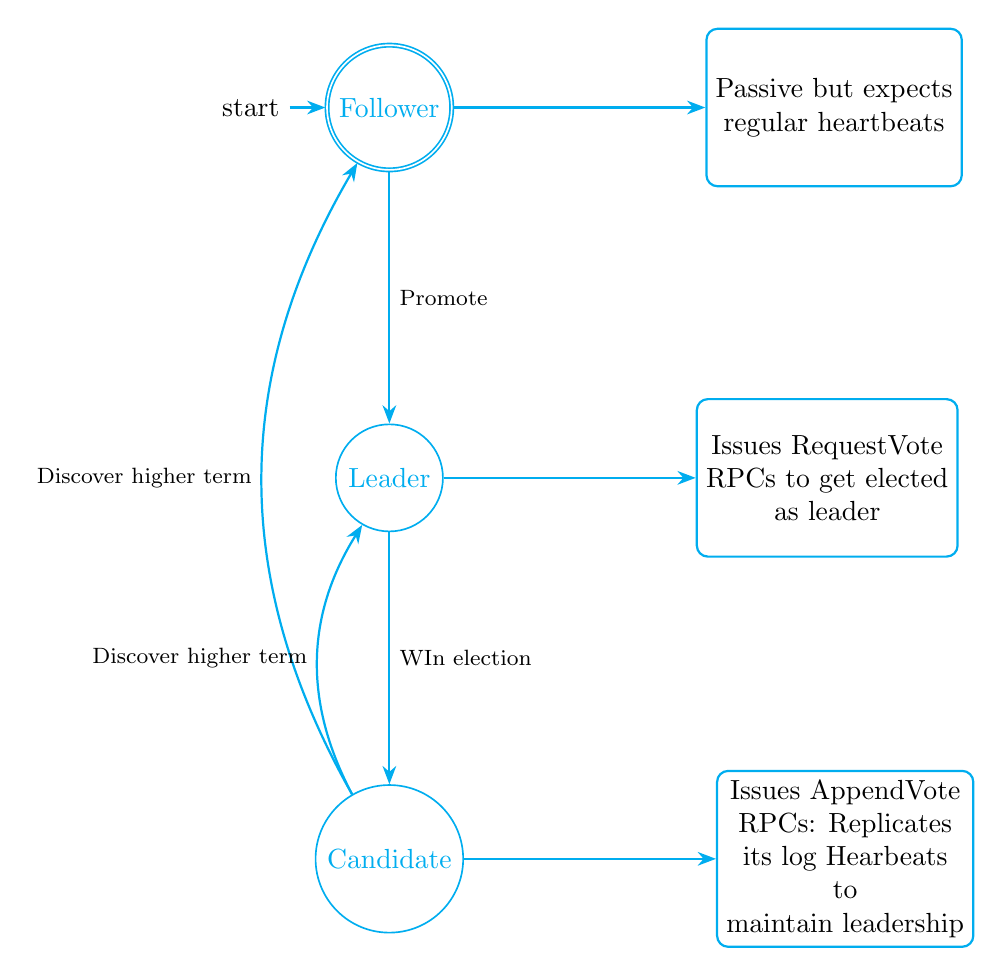
\begin{tikzpicture}[auto,
            > = Stealth,
every edge quotes/.style = {font=\footnotesize}, % if you like to have smaller edge labels
every edge/.append style = {->, draw=cyan, thick},
every loop/.append style = {<-, looseness = 12},
node distance = 32mm,
 state/.style = {circle, semithick, draw=cyan, text=cyan, minimum size=1.2em},
      rect/.style = {rectangle, draw=cyan, thick, minimum width=2.5cm, minimum height=1.5cm, align=center}
]
\node (A) [state, initial, accepting]   {Follower};
\node (B) [state, below=of A]           {Leader};
\node (C) [state, below=of B]           {Candidate};
\node (A1)  [rect,rounded corners,right=of A,draw,thick,minimum width=2cm,minimum height=2cm] {Passive but expects \\ regular heartbeats};
\node (B1)  [rect,rounded corners, right=of B,draw,thick,minimum width=2cm,minimum height=2cm] {Issues RequestVote \\RPCs  to get elected \\as leader};
\node (C1)  [rect,rounded corners,right=of C,draw,thick,minimum width=2cm,minimum height=2cm] {Issues AppendVote\\RPCs: Replicates \\its log Hearbeats \\to \\maintain leadership};
\path
        (C) edge [bend left,"Discover higher term"]     (A)
        (C) edge [bend left,"Discover higher term"]     (B)
        (A) edge ["Promote"]     (B)
        (B) edge [ "WIn election"]   (C)
        (A) edge [ right]   (A1)
        (B) edge [ right]  (B1)
        (C) edge [ right]  (C1);

\end{tikzpicture}
\eject

\vspace{5500px}
\usetikzlibrary{fit,positioning,calc,arrows,backgrounds}
\tikzset{
    my1/.style={
        draw=gray,thick,fill=gray!40,minimum height=1.5cm,minimum width=1.5cm,align=center,text width=4.8cm,font={\Huge\bfseries}
    },
    my/.style={
        draw=gray,thick,fill=gray!40,minimum height=1.5cm,minimum width=1.5cm,font={\Huge\bfseries}
    },
    >=latex
}
    \begin{tikzpicture}[font=\sffamily, node distance=0.2cm and 0.2cm]
        \node[my] (b11) {$b_1$};
        \node[my,right=of b11] (b12) {$b_2$};
        \node[my,right=of b12] (b13) {$b_3$};
        \node[my,right=of b13] (b14) {$b_4$};
        \node[my,right=of b14] (b15) {};
        \node[my,right=of b15] (b16) {};
        \node[my,right=of b16] (b17) {};
        \node[my,right=of b17] (b18) {};
        \begin{pgfonlayer}{background}
            \node[draw=black,thick,fill=gray!30,fit=(b11)] {};
            \node[draw=black,thick,fill=gray!30,fit=(b12)]  {};
            \node[my1,anchor=west] at (0,3) (pk){4 Partial\\Keys\strut};
            \node[draw=black,thick,fill=gray!30,fit=(b13)] {};
            \node[draw=black,thick,fill=gray!30,fit=(b14)] {};
            \node[draw=black,thick,fit=(b15)] {};
            \node[draw=black,thick,fit=(b16)] {};
            \node[draw=black,thick,fit=(b17)] {};
            \node[draw=black,thick,fit=(b18)] {};
            \draw[->, black,thick] (b15) -- ++(0,-3);
            \draw[->, black,thick] (b16) -- ++(0,-3);
            \draw[->, black,thick] (b17) -- ++(0,-3);
            \node[my1,anchor=west] at (6,3) {4 Child\\Pointers\strut};
            \draw[->, black,thick] (b18) -- ++(0,-3);
        \end{pgfonlayer}
        \begin{scope}[xshift=6cm]
            \begin{pgfonlayer}{background}
            \end{pgfonlayer}
        \end{scope}
\node [font = {\Huge\bfseries\sffamily},
       above right=of pk] (t0) {Node\_4};
\end{tikzpicture}
\pgfplotsset{compat=1.18}
    \usetikzlibrary{fit,positioning,calc,backgrounds,shapes.geometric,arrows.meta}

    \tikzset{
      my1/.style={
        draw=gray,thick,fill=gray!40,
        minimum height=1.5cm,minimum width=1.5cm,align=center,text width=4.8cm,
        font={\Huge\bfseries}
      },
      my/.style={
        draw=gray,thick,fill=gray!40,
        minimum height=1.5cm,minimum width=1.5cm,align=center,
        font={\Huge\bfseries}
      },
      dots/.style={
        draw=none,fill=none,
        minimum height=1.5cm,
        minimum width=1.0cm,
        inner sep=0pt,
        font={\Huge\bfseries}
      },
      >=Latex
    }

    
    \begin{tikzpicture}[font=\sffamily, node distance=0.2cm and 0.2cm]

      % --- Partial keys
      \node[my] (b111) {$b_1$};
      \node[my,right=of b111] (b112) {$b_2$};
      \node[my,right=of b112] (b113) {$b_3$};
      \node[my,right=of b113] (b114) {$b_4$};

      % ellipsis between b4 and bn
      \node[dots,right=of b114] (dotskey) {$\cdots$};

      % IMPORTANT: unique name (bnkey), do not reuse (bn) later
      \node[my,right=of dotskey] (bnkey) {$b_n$};

      % --- Child pointers (empty boxes)
      \node[my,right=of bnkey] (p115) {};
      \node[my,right=of p115] (p116) {};
      \node[my,right=of p116] (p117) {};
      \node[my,right=of p117] (p118) {};

      % ellipsis between 4th and last pointer boxes
      \node[dots,right=of p118] (dotsptr) {$\cdots$};

      % IMPORTANT: unique name (bnptr)
      \node[my,right=of dotsptr] (bnptr) {};

      \begin{pgfonlayer}{background}
        % Labels (as in your code)
        \node[my1,anchor=west] at (0,3) (pk1){16 Partial\\Keys\strut};
        \node[my1,anchor=west] at (6,3) {16 Child\\Pointers\strut};

        % Frames/backgrounds for key boxes
        \node[draw=black,thick,fill=gray!30,fit=(b111)] {};
        \node[draw=black,thick,fill=gray!30,fit=(b112)] {};
        \node[draw=black,thick,fill=gray!30,fit=(b113)] {};
        \node[draw=black,thick,fill=gray!30,fit=(b114)] {};
        \node[draw=black,thick,fill=gray!30,fit=(bnkey)] {};
        \node[draw=black,thick,fill=gray!30,fit=(dotskey)] {}; % <--
        \node[draw=black,thick,fill=gray!30,fit=(dotsptr)] {}; % <--

        % Frames for pointer boxes
        \node[draw=black,thick,fit=(p115)] {};
        \node[draw=black,thick,fit=(p116)] {};
        \node[draw=black,thick,fit=(p117)] {};
        \node[draw=black,thick,fit=(p118)] {};
        \node[draw=black,thick,fit=(bnptr)] {};

        % Arrows
        \draw[->, black,thick] (p115) -- ++(0,-3);
        \draw[->, black,thick] (p116) -- ++(0,-3);
        \draw[->, black,thick] (p117) -- ++(0,-3);
        \draw[->, black,thick] (p118) -- ++(0,-3);
        \draw[->, black,thick] (bnptr) -- ++(0,-3);
      \end{pgfonlayer}

      \node[font={\Huge\bfseries\sffamily}, above right=of pk1] (t1) {Node\_16};

    \end{tikzpicture}

    \begin{tikzpicture}[font=\sffamily, ar/.style={->,>=latex},node distance=0.2cm and 0.2cm]

      \node[my] (b111) {$b_1$};
      \node[my,right=of b111] (b112) {$b_2$};
      \node[my,right=of b112] (b113) {$b_3$};
      \node[my,right=of b113] (b114) {$b_4$};

      \node[dots,right=of b114] (dotskey) {$\cdots$};

      \node[my,right=of dotskey] (bnkey) {$b_n$};

      % --- Child pointers (empty boxes)
      \node[my,right=of bnkey] (p115) {};
      \node[my,right=of p115] (p116) {};
      \node[my,right=of p116] (p117) {};
      \node[my,right=of p117] (p118) {};

      % ellipsis between 4th and last pointer boxes
      \node[dots,right=of p118] (dotsptr) {$\cdots$};

      % IMPORTANT: unique name (bnptr)
      \node[my,right=of dotsptr] (bnptr) {};

      \begin{pgfonlayer}{background}
        % Labels (as in your code)
        \node[my,anchor=west] at (0,3) (pk1){ Child Index\strut};
        \node[my,anchor=west] at (6,3) { Child Pointers\strut};

        % Frames/backgrounds for key boxes
        \node[draw=black,thick,fill=gray!30,fit=(b111)] (ar1)  {};
        \node[draw=black,thick,fill=gray!30,fit=(b112)] {};
        \node[draw=black,thick,fill=gray!30,fit=(b113)] {};
        \node[draw=black,thick,fill=gray!30,fit=(b114)] {};
        \node[draw=black,thick,fill=gray!30,fit=(bnkey)] {};
        \node[draw=black,thick,fill=gray!30,fit=(dotskey)] {}; % <--
        \node[draw=black,thick,fill=gray!30,fit=(dotsptr)] {}; % <--

        % Frames for pointer boxes
        \node[draw=black,thick,fit=(p115)] (ar2) {};
        \node[draw=black,thick,fit=(p116)] {};
        \node[draw=black,thick,fit=(p117)] {};
        \node[draw=black,thick,fit=(p118)] {};
        \node[draw=black,thick,fit=(bnptr)] {};

        % Arrows
        \draw[->, black,thick] (p115) -- ++(0,-3);
        \draw[->, black,thick] (p116) -- ++(0,-3);
        \draw[->, black,thick] (p117) -- ++(0,-3);
        \draw[->, black,thick] (p118) -- ++(0,-3);
        \draw[->, black,thick] (bnptr) -- ++(0,-3);
      \end{pgfonlayer}

        \draw (b111.north) edge[-{Stealth[scale=3]},dotted,ultra thick,bend left=25] (p116.north);
        \draw (b112.north) edge[-{Stealth[scale=3]},dotted,ultra thick,bend left=25] (p115.north);
        \draw (b113.north) edge[-{Stealth[scale=3]},dotted,ultra thick,bend left=25] (p118.north);
        \draw (b114.north) edge[-{Stealth[scale=3]},dotted,ultra thick,bend left=25] (p117.north);
        \draw (bnkey.north) edge[-{Stealth[scale=3]},dotted,ultra thick,bend left=25] (bnptr.north);

      \node[font={\Huge\bfseries\sffamily}, above right=of pk1] (t1) {Node\_48};


    \end{tikzpicture}
    \begin{tikzpicture}[font=\sffamily, ar/.style={->,>=latex},node distance=0.2cm and 0.2cm]

      \node[my] (b111) {$0$};
      \node[my,right=of b111] (b112) {$1$};
      \node[my,right=of b112] (b113) {$2$};
      \node[my,right=of b113] (b114) {$3$};
      \node[my,right=of b114] (b115) {$4$};
      \node[my,right=of b115] (b116) {$5$};
      \node[my,right=of b116] (b117) {$6$};

      \node[dots,right=of b117] (dotskey) {$\cdots$};

      \node[my,right=of dotskey] (bnkey) {$255$};



      \begin{pgfonlayer}{background}
        % Labels (as in your code)
        \node[my,anchor=west] at (0,3) (pk1){ Child Pointer\strut};

        % Frames/backgrounds for key boxes
        \node[draw=black,thick,fill=gray!30,fit=(b111)] (ar1)  {};
        \node[draw=black,thick,fill=gray!30,fit=(b112)] {};
        \node[draw=black,thick,fill=gray!30,fit=(b113)] {};
        \node[draw=black,thick,fill=gray!30,fit=(b114)] {};
        \node[draw=black,thick,fill=gray!30,fit=(b115)] {};
        \node[draw=black,thick,fill=gray!30,fit=(b116)] {};
        \node[draw=black,thick,fill=gray!30,fit=(b117)] {};
        \node[draw=black,thick,fill=gray!30,fit=(bnkey)] {};
        \node[draw=black,thick,fill=gray!30,fit=(dotskey)] {}; % <--

      \end{pgfonlayer}


      \node[font={\Huge\bfseries\sffamily}, above right=of b114] (t1) {Node\_256};

    \end{tikzpicture}




\vspace*{7cm}\par

\begin{forest}
for tree = {
  every node/.style={minimum size=4mm, inner sep=0.5mm},
  normal/.style={circle,draw,
            minimum size=1.5em, % <-- added
            inner sep=1pt},      % <-- added
  invis/.style={draw=none},
  border/.style={ edge from parent/.style={dashed,draw} },
  acc/.style={circle,very thick,font=\small\bfseries,
            minimum size=1.5em, % <-- added
            inner sep=1pt,      % <-- added
            draw=gray!70},
  rej/.style={rectangle,very thick,font=\small\bfseries,
            minimum size=1.5em, % <-- added
            inner sep=1pt,      % <-- added
            draw=gray!70},
  rem/.style={circle,thick,draw=gray!70,
            minimum size=1.5em, % <-- added
            inner sep=1pt},      % <-- added
  semithick,
  where n children=0{tier=bottom}{}
}
[0, acc
  [0, acc, name = L1, for descendants=border
    [0, acc
      [1, acc
        [0, acc, name = L3
        [a, rej, name = L4,tier=bottom]
        [-, phantom]
        ]
        [-, phantom]
      ]
      [1, rem, name = L6
        [-, phantom]
        [1, rem, name = L7
        [b, rej, name = L5,tier=bottom]
        [-, phantom]]
      ]
    ]
    [-, phantom]
  ]
  [-, phantom]
]
\end{forest}

%% \begin{tikzpicture}[every text node part/.style={align=left},
%% %%                      stack/.style={rectangle split,
%%                                    rectangle split parts = 5,
%%                                    draw,text width=1.5cm},
%%                     myarrow/.style={single arrow,
%%                                     draw,
%%                                     right = 3pt,
%%                                     minimum size = 5ex}
%%                   ]

%% % we start
%% \node [stack] (ini)  {%
%%                       $a=0$     \nodepart{two}
%%                       $b=10$    \nodepart{three}
%%                       $c=100$   \nodepart{four}
%%                       $d=-10$   \nodepart{five}
%%                       $\cdots$};
%% % we add an arrow
%% \node [myarrow] (A) at (ini.east) {} ;
%% % after the arrow, the main node at the end
%% \node [draw,rectangle,align=left,right=3pt] (mid) at (A.east)
%%             {instruction 0;\\
%%              instruction 1;\\
%%              $\ldots$\\
%%              instruction $n$;};
%% % we add another arrow
%% \node [myarrow] (B) at (mid.east) {} ;
%% % after the arrow, the final node
%% \node [stack,right=3pt] (fin) at (B.east)  {%
%%                                             $a=10$    \nodepart{two}
%%                                             $b=100$   \nodepart{three}
%%                                             $c=-10$   \nodepart{four}
%%                                             $d=110$   \nodepart{five}
%%                                             $\cdots$};
%% % labels : I don't like vey much `label= ` it's a shortcut but I think it's more powerful and flexible to use real nodes.
%% \node [above,align=left]  at (ini.north) {Initial values of\\
%%                                           variables};
%% \node [above,align=left]  at (fin.north) {Final values of\\
%%                                           variables};
%% \node [above]             at (mid.north) {Computer Program};


%% \end{tikzpicture}

%% \begin{tikzpicture}[
%%     every node/.style={
%%         draw,minimum width=1in,
%%         text height=1.75ex,
%%         text depth=0.5ex,
%%     },
%%     node distance=-\pgflinewidth,
%% ]
%%     \node (b0) {$b_0$};
%%     \node (b1) [right=of b0] {$b_1$};
%%     \node (b2) [right=of b1] {$b_2$};
%%     \node (dots) [right=of b2] {$\cdots$};
%%     \node (bSt) [right=of dots] {$b_{S.t}$};
%% \matrix (tbl) [below=2cm of b0, row sep=0pt, column sep=0pt] {
%%     \node[ TBox ] (checksum)  {checksum}; &
%%     \node[ TBox ]  (key)       {key}; &
%%     \node[ TBox ] (value)    {value}; &
%%     \node[ TBox ] (deleted)  {deleted}; &
%%     \node[ TBox ] (offset)   {offset}; &
%%     \node[ TBox ]  (size)      {size}; &
%%     \node[ TBox ] (tstamp)   {tstamp}; &
%%     \node[ TBox ] (keysize)  {keysize}; &
%%     \node[ TBox ] (valuesize){valuesize}; \\
%% };


%%     \draw[red,->, thick] (bSt.south) -- (key.north);

%% \end{tikzpicture}
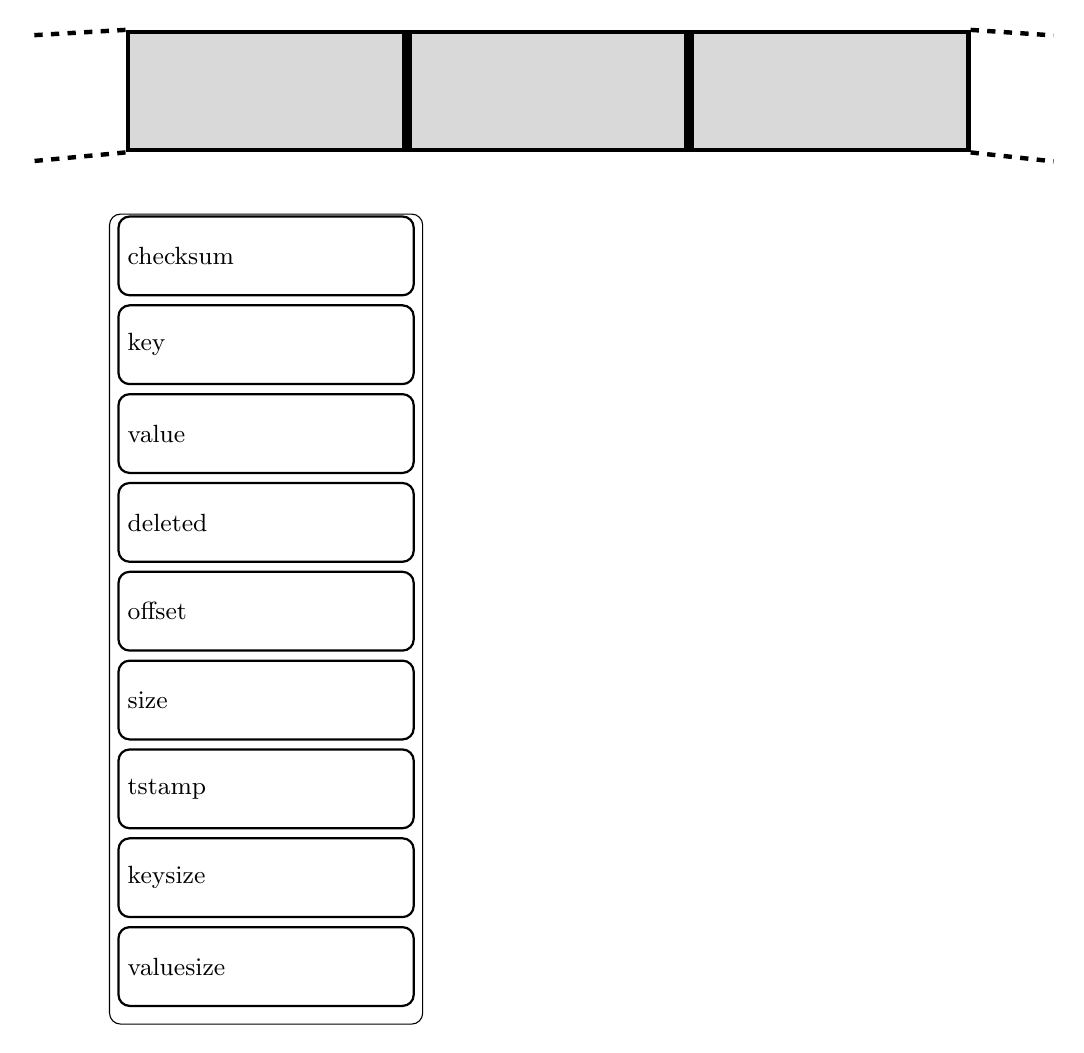
\begin{tikzpicture}[
node distance = 1mm and 6mm,
  start chain = going below,
box/.style = {draw, thick, rounded corners,
              text width=10em, align=left, minimum height=1cm,
              font=\small,
              on chain},
FITout/.style args={#1}{
    box,
    thin,
    inner xsep=1mm,
    inner ysep=6mm,
    yshift=12mm,
    fit=#1
},
emptybox/.style = {
        draw,ultra thick, minimum width=10em,
        minimum height=15mm
    },
FITinn/.style = {FITout=#1,inner ysep=3mm, yshift=-2mm},
every label/.style = {text width=11em, align=center,
                      font=\small\linespread{0.84}\selectfont}
                ]
%% \framebox[60mm]{\rule{0pt}{40mm}}

\node (p1) [box] {checksum};
\node (p2) [box] {key};
\node (p3) [box] {value};
\node (p4) [box] {deleted};
\node (p5) [box] {offset};
    \node(p6)  [box]      {size};
    \node(p7) [box]   {tstamp};
    \node(p8) [box]  {keysize};
    \node(p9) [box]{valuesize};
\node (h1) [emptybox,fill=gray!30, above=8mm of p1] {};
\node (h2) [emptybox,fill=gray!30, right=0.1mm of h1] {};
\node (h3) [emptybox,fill=gray!30, right=0.1mm of h2] {};
\draw [ultra thick, dashed] (h3.north east) -- (10,2.8);
\draw [ultra thick, dashed] (h3.south east) -- (10,1.2);
\draw [ultra thick, dashed] (h1.north west) -- (-3,2.8);
\draw [ultra thick, dashed] (h1.south west) -- (-3,1.2);
\node[box, thin, inner xsep=1mm,
      fit={(p1) (p9)}] (x1) {};
%%
\end{tikzpicture}
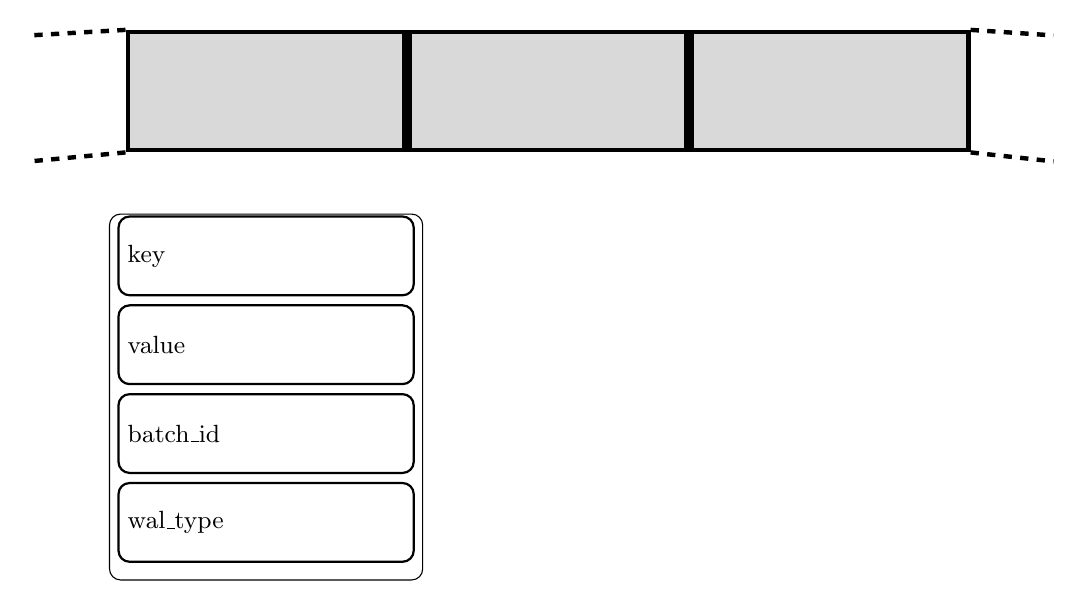
\begin{tikzpicture}[
node distance = 1mm and 6mm,
  start chain = going below,
box/.style = {draw, thick, rounded corners,
              text width=10em, align=left, minimum height=1cm,
              font=\small,
              on chain},
FITout/.style args={#1}{
    box,
    thin,
    inner xsep=1mm,
    inner ysep=6mm,
    yshift=12mm,
    fit=#1
},
emptybox/.style = {
        draw,ultra thick, minimum width=10em,
        minimum height=15mm
    },
FITinn/.style = {FITout=#1,inner ysep=3mm, yshift=-2mm},
every label/.style = {text width=11em, align=center,
                      font=\small\linespread{0.84}\selectfont}
                ]
%% \framebox[60mm]{\rule{0pt}{40mm}}

\node (p1) [box] {key};
\node (p2) [box] {value};
\node (p3) [box] {batch\_id};
\node (p4) [box] {wal\_type};
\node (h1) [emptybox,fill=gray!30, above=8mm of p1] {};
\node (h2) [emptybox,fill=gray!30, right=0.1mm of h1] {};
\node (h3) [emptybox,fill=gray!30, right=0.1mm of h2] {};
\draw [ultra thick, dashed] (h3.north east) -- (10,2.8);
\draw [ultra thick, dashed] (h3.south east) -- (10,1.2);
\draw [ultra thick, dashed] (h1.north west) -- (-3,2.8);
\draw [ultra thick, dashed] (h1.south west) -- (-3,1.2);
\node[box, thin, inner xsep=1mm,
      fit={(p1) (p4)}] (wal) {};
%%
\end{tikzpicture}
\begin{tikzpicture}
%%   \begin{axis}[grid=both,ymin=-5,ymax=5,xmax=5,xmin=-5,xticklabel=\empty,yticklabel=\empty,
%%                minor tick num=1,axis lines = middle,xlabel=$x$,ylabel=$y$,label style =
%%                {at={(ticklabel cs:1.1)}},
%% legend style={font=\small},
%% legend cell align=left,        % <---
%% legend pos=north west,
%%     ]
%% \addplot[
%%     color=cyan,
%%     mark=square,
%%     ]
%%     coordinates {
%%     (0,0)(1,1)
%%     };
%% \addplot[
%%     color=red,
%%     mark=square,
%%     ]
%%     coordinates {
%%     (1,0)(0,1)
%%     };

%% \addplot[
%%     color=blue,
%%     mark=square,
%%     ]
%%     coordinates {
%%     (1,1)(1,0)
%%     };
%% \legend{$\alpha_t$,$\beta_t$,}
%%   \end{axis}
%% \end{tikzpicture}
 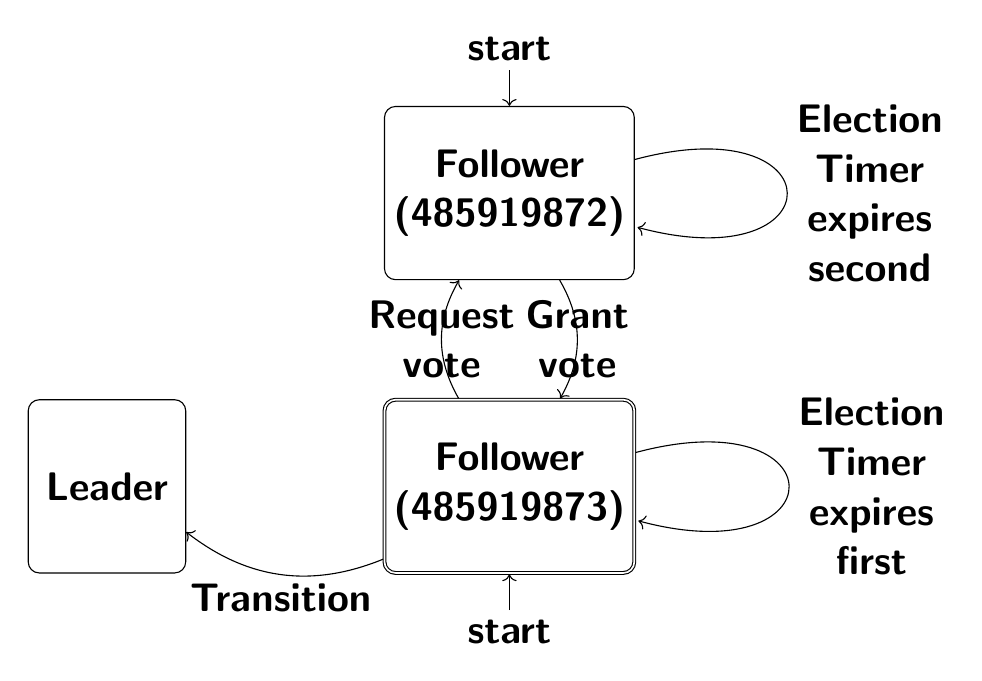
\begin{tikzpicture}[
    every state/.style={
        draw,font={\Large\bfseries\sffamily},
        rectangle,
        rounded corners,
        minimum width=2cm,
        minimum height=2.2cm, % This will now work
        align=center
    },
every node/.style={
        font=\Large\bfseries\sffamily
    },
    node distance=1.5cm and 2.5cm
]
\node[state, initial, initial where=below, accepting] (123) {Follower\\(485919873)};
\node[state, initial, initial where=above, above=of 123] (2) {Follower\\(485919872)};
\node[state, left=of 123] (23) {Leader};
\draw [->]

(123) edge[bend left] node[align=center] {Request\\vote} (2)
(2) edge[bend left] node[align=center] {Grant\\vote} (123)

(123) edge[loop right] node[align=center] {Election\\Timer\\expires\\first} (123)
(2) edge[loop right] node[align=center] {Election\\Timer\\expires\\second} (2)
(123) edge[bend left,below] node {Transition} (23);
\end{tikzpicture}
    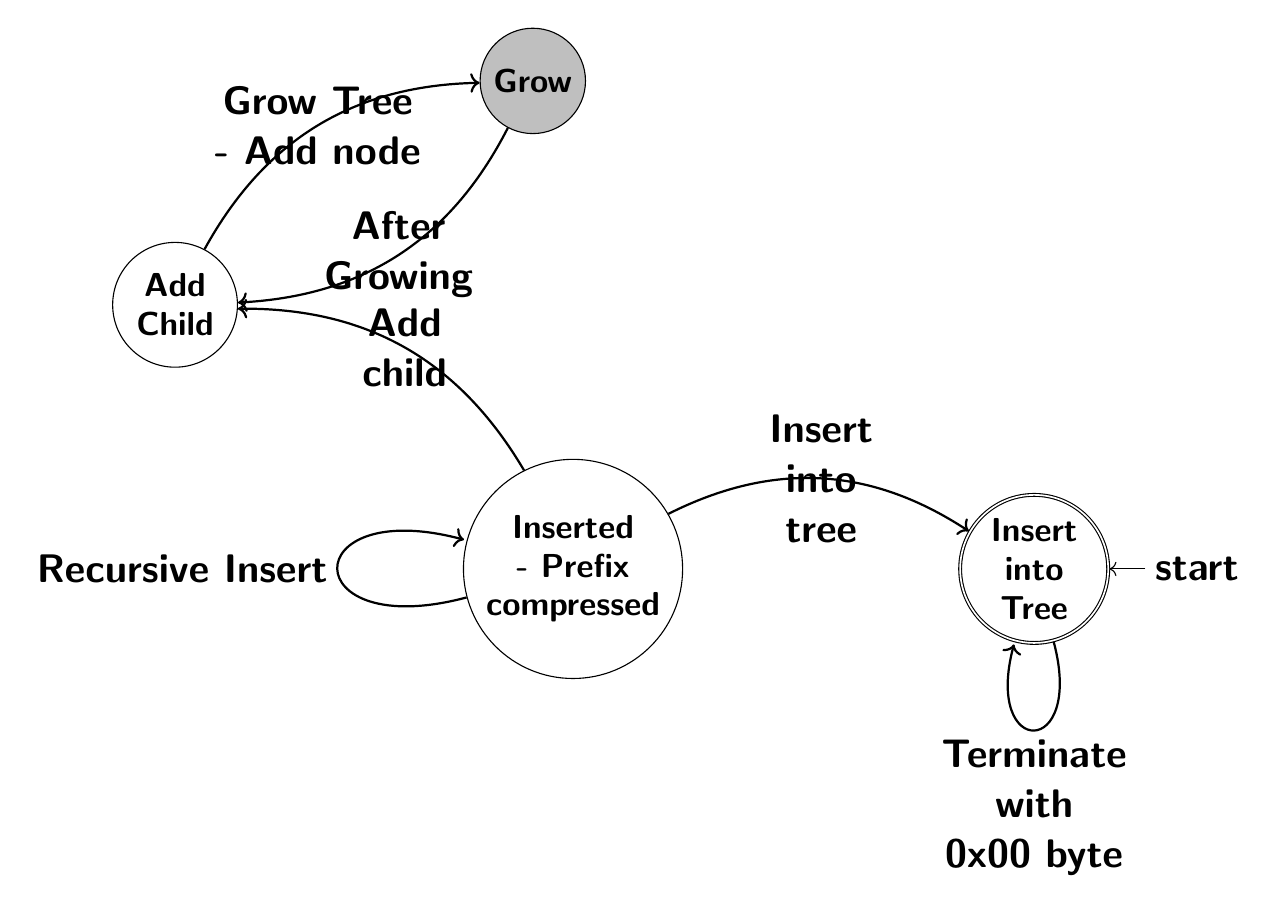
\begin{tikzpicture}[
every node/.style={
        font=\Large\bfseries\sffamily
    },
node distance = 18mm and 35mm,
    MP/.style = {circle, draw, inner sep=2pt,
                 align=center,  font=\large\bfseries\sffamily},
state/.append style = {fill=#1,font=\large\bfseries\sffamily, align=center},
state/.default = white,
every edge quotes/.append style={ align=center,  font=\large\bfseries\sffamily, auto}% style for edge labels
    ]
\node (Addchild)    [state]   {Add\\Child};
\node (Grow)        [state=gray!50, above right=of Addchild] {Grow};
\node (Insert) [MP, below right=of Addchild]
        {Inserted\\- Prefix\\compressed};

\node (Treeinsert) [MP, initial, initial where=right, accepting,right=of Insert]
        {Insert\\into\\Tree};

%\scoped[on background layer]
%% \node  (digital) [rounded corners, draw=red, label=75:Digital state,
%%                   fit=(Digital Off) (Digital On)] {};
\path[thick, ->]
    (Addchild)      edge [bend  left]  node[align=center] {Grow Tree\\- Add node} (Grow)
    (Grow)          edge [bend left]  node[align=center] {After\\Growing}  (Addchild)
    (Insert)   edge [loop left] node[align=center] {Recursive Insert} (Insert)
    (Insert)    edge [bend left] node[align=center] {Insert\\into\\tree} (Treeinsert)
    (Treeinsert) edge[loop below] node[align=center] {Terminate\\with\\0x00 byte} (Treeinsert)
    (Insert)       edge [bend right] node[align=center] {Add\\child} (Addchild);
    \end{tikzpicture}


% ~~~~~~~~~~~~~~~~~~~~~~~~~~~~~~~~~
\newcommand\cntnt[2]{%      content
        \textbf{#1}%
        \nodepart{second}%
        #2}


 %% \begin{tikzpicture}[
 %%    >={Latex[length=3mm]},      % replacing all arrow tips
 %%    pn/.style={anchor=north,yshift=-1mm},   % for path nodes/notes
 %%    pnr/.style={anchor=west,xshift= 1mm},
 %%    labelnode/.style={
 %%        font=\large\bfseries\sffamily,
 %%        rectangle split,
 %%        rectangle split parts=2,
 %%        draw=black!80,
 %%        rounded corners,
 %%        fill=gray!5,
 %%        align=center,
 %%        inner sep=3pt,
 %%        minimum width=2.5cm,    % changed
 %%        anchor=north,           % "align" at top
 %%    },
 %%    % Infeasible (MS Pruning) - Rot
 %%    infeasible/.style={
 %%        labelnode,
 %%        draw=red!80,
 %%        fill=red!5,
 %%        dashed
 %%    },
 %%    % Dominated (History Dominance) - Lila
 %%    dominated/.style={
 %%        infeasible,     % kind of css-approach
 %%        draw=violet!80,
 %%        fill=violet!5,
 %%    },
 %%    % Optimal Path Node - Grün
 %%    optimal/.style={
 %%        labelnode,
 %%        draw=green!50!black,
 %%        fill=green!10,
 %%        line width=1pt
 %%    },
 %%    worker/.style=      {->, blue!70!black, thick},
 %%    ai/.style=          {->, orange!80!black, thick},
 %%    optedge/.style=     {worker, line width=1.5pt, green!40!black},
 %%    prunededge/.style=  {->, red!70, dashed},
 %%    domedge/.style=     {->, violet!70,},% dashed},
 %%    tl/.style=          {->, thick, gray,anchor=west}, % timeline
 %%    ltl/.style=         {gray, anchor=south}, % label for timelin
 %% ]
 %%    % ~~~ placing nodes ~~~~~~~~~~~~~~~~~
 %%    \matrix[                    % this works much like a table
 %%            column sep= 20mm,   % chose as needed
 %%            row sep   = 10mm,
 %%    ]
 %%    {   % all those nodes
 %%        % ~~~ row 1 ~~~~~~~~~~~~~~
 %%        \node[labelnode,yshift=-2mm]
 %%                        (a){\cntnt{Start}       {$V=0, \omega=0$}};                 &
 %%        \node[optimal]  (b){\cntnt{W1}      {$V=3, \omega=1.0$\\$h=[1]$}};      &
 %%        \node[optimal]  (c){\cntnt{W $\to$ W}   {$V=6, \omega=2.0$\\$h=[1,1]$}};    &
 %%        \node[optimal]  (d){\cntnt{3 Workers}   {$V=9, \omega=3.0$\\Target met}};   \\
 %%        % ~~~ row 2 ~~~~~~~~~~~~~~
 %%        &&\node[dominated] (e){\cntnt{W $\to$ AI}{Dominated\\
 %%                                               $V=4, \omega=1.3$\\$h=[1,0]$}};  \\
 %%        % ~~~ row 3 ~~~~~~~~~~~~~~
 %%        & \node[labelnode](f){\cntnt{A1}        {$V=1, \omega=0.3$\\$h=[0]$}};      &
 %%        \node[labelnode]  (g){\cntnt{A1 $\to$ W}{$V=4, \omega=1.3$\\$h=[0,1]$}};    \\
 %%        % ~~~ row 4 ~~~~~~~~~~~~~~
 %%        &&\node[infeasible](h){\cntnt{A1 $\to$ AI}{Pruned\\$h=[0,1]$}};             \\
 %%    };

 %%    % ~~~ connections ~~~~~~~~~~~~~~~~~~~~~~~~~~
 %%    % ~~~ row 1 ~~~~~~~~~~~~~~~~
 %%    \draw[optedge]      (a) -- node[pn]{W (+3)} (b);
 %%    \draw[optedge]      (b) -- node[pn]{W (+3)} (c);
 %%    \draw[optedge]      (c) -- node[pn]{W (+3)} (d);
 %%    % ~~~ row 3 ~~~~~~~~~~~~~~~~
 %%    \draw[worker]       (f) -- node[pn]{W (+3)} (g);
 %%    % ~~~ other ~~~~~~~~~~~~~~~~
 %%    \draw[domedge]      (g) -- node[pnr]{Dominance Check}   (e);
 %%    \draw[prunededge]   (f) |- node[pn,pos=.75]{Violation}(h);
 %%    \draw[ai]           (a) |- node[pn,pos=.8]{AI (+1)}(f);
 %%    \draw[ai]           (b) |- node[pn,pos=.7]{AI (+1)}(e);

 %%    % ~~~ timeline ~~~~~~~~~~~~
 %%    \coordinate (R) at ([yshift=5mm]d.north east);  % lift it a little
 %%    \coordinate (L) at (a.north west |- R);         % intersection, as "Start" is shifted

 %%    \draw[tl] (L) -- (R) node {Time $t$};
 %%    \foreach \n/\t in {a/0, b/1, c/2, d/3}          % just being lazy
 %%        \node[ltl] at (\n |- L) {$t=\t$};


 %% \end{tikzpicture}
\tikzset{
    font=\tt,
    >= stealth,
    every picture/.style={thick},
    pointer/.style={*->},
    every node/.style={
        font=\Large\bfseries\sffamily
    },
    node/.style={
        rounded corners,
        minimum width=2.5cm,
        minimum height=2cm,
        align=center,
        rectangle split, rectangle split horizontal,
        rectangle split parts=#1,
        draw,
        anchor=center,
        rectangle split part align={center},
        every twelve node part/.style={font=\itshape, align=center},
        rectangle split empty part width=1.5
    }
}
\tikzstyle{stuff_fill}=[rectangle,draw,fill=black!20,rounded corners=3pt,inner sep=4pt]
\begin{tikzpicture}[remember picture]
%% \node[
%%   draw=gray!50,
%%   fill=gray!08,
%%   rounded corners=4pt,
%%   inner sep=6pt,
%%   line width=0.6pt
%% ]{
     \node[node=5,
        rectangle split part fill={gray!40,gray!40,gray!40,white,white}
    ] (A) {
        \nodepart{one}[]
        \nodepart{two}2
        \nodepart{three}0
        \nodepart{four}h
        \nodepart{five}y
    };
%% };

    \node[node=12,draw,  rectangle split part fill={white,white,white,white,white,white,white,white,white,white,white},below=6cm of A] (B) {
        \nodepart{one}h
        \nodepart{two}e
        \nodepart{three}l
        \nodepart{four}l
        \nodepart{five}o
        \nodepart{six}w
        \nodepart{seven}o
        \nodepart{eight}r
        \nodepart{nine}l
        \nodepart{ten}d
        \nodepart{eleven}0x00
        \nodepart{twelve}1L
    };
%% \node[
%%   draw=gray!50,
%%   fill=gray!08,
%%   rounded corners=4pt,
%%   inner sep=6pt,
%%   line width=0.6pt
%% ]{
     \node[node=6,draw,  rectangle split part fill={gray!40,gray!40,gray!40,white,white,white},below right =1.4cm of A] (D) {
        \nodepart{one}o
        \nodepart{two}3
        \nodepart{three}1
        \nodepart{four}e
        \nodepart{five}l
        \nodepart{six}p
    };
%% };

    \node[node=9,draw,  rectangle split part fill={white,white,white,white,white,white,white,white,white},below right=5cm of A] (C) {
        \nodepart{one}y
        \nodepart{two}o
        \nodepart{three}e
        \nodepart{four}a
        \nodepart{five}r
        \nodepart{six}t
        \nodepart{seven}h
        \nodepart{eight}0x00
        \nodepart{nine}{\normalfont\textit{2L}}
    };

\node[
  stuff_fill,
  left=0.5cm of D,
  text width=3cm,
  align=center
] {Common prefix\\is extracted};
\draw[->,bend right=40]
  ($(A.four)+(0,-0.3)$)
  to
  ($(B.one)+(0,0.3)$);
\draw[->]
  ($(A.five)+(0,-0.3)$)
  --
  ($(D.four)+(0,0.3)$);
\draw[->]
  ($(D.four)+(0,-0.3)$)
  --
  ($(C.one)+(0,0.3)$);
\node[gray!80] at ($(A.one)!0.5!(A.three)+(0,0.6)$) {Prefix};
\node[gray!80] at ($(D.one)!0.5!(D.three)+(0,0.6)$) {Prefix};

\end{tikzpicture}

%% \tikzset{
%%     font=\tt,
%%     >= stealth,
%%     every picture/.style={thick},
%%     pointer/.style={*->},
%%     every node/.style={
%%         font=\Large\bfseries\sffamily
%%     },
%%     node/.style={
%%         rounded corners,
%%         minimum width=2.5cm,
%%         minimum height=2cm,
%%         align=center,
%%         rectangle split, rectangle split horizontal,
%%         rectangle split parts=#1,
%%         draw,
%%         anchor=center,
%%         rectangle split part align={center},
%%         every twelve node part/.style={font=\itshape, align=center},
%%         rectangle split empty part width=1.5
%%     }
%% }
%% \tikzstyle{stuff_fill}=[rectangle,draw,fill=black!20,rounded corners=3pt,inner sep=4pt]
%% \begin{tikzpicture}[remember picture]
%%      \node[node=5,
%%         rectangle split part fill={gray!40,gray!40,gray!40,white,white}
%%     ] (A) {
%%         \nodepart{one}[]
%%         \nodepart{two}2
%%         \nodepart{three}0
%%         \nodepart{four}h
%%         \nodepart{five}y
%%     };
%% %% };

%%     \node[node=12,draw,  rectangle split part fill={white,white,white,white,white,white,white,white,white,white,white},below=8cm of A] (B) {
%%         \nodepart{one}h
%%         \nodepart{two}e
%%         \nodepart{three}l
%%         \nodepart{four}l
%%         \nodepart{five}o
%%         \nodepart{six}w
%%         \nodepart{seven}o
%%         \nodepart{eight}r
%%         \nodepart{nine}l
%%         \nodepart{ten}d
%%         \nodepart{eleven}0x00
%%         \nodepart{twelve}1L
%%     };
%% %% \node[
%% %%   draw=gray!50,
%% %%   fill=gray!08,
%% %%   rounded corners=4pt,
%% %%   inner sep=6pt,
%% %%   line width=0.6pt
%% %% ]{
%%      \node[node=6,draw,  rectangle split part fill={gray!40,gray!40,gray!40,white,white,white},below right =1.4cm of A] (D) {
%%         \nodepart{one}o
%%         \nodepart{two}3
%%         \nodepart{three}1
%%         \nodepart{four}e
%%         \nodepart{five}l
%%         \nodepart{six}p
%%     };
%% %% };

%%     \node[node=10,draw,  rectangle split part fill={white,white,white,white,white,white,white,white,white},below right=4.6cm of A] (E) {
%%         \nodepart{one}y
%%         \nodepart{two}o
%%         \nodepart{three}l
%%         \nodepart{four}e
%%         \nodepart{five}a
%%         \nodepart{six}r
%%         \nodepart{seven}t
%%         \nodepart{eight}h
%%         \nodepart{nine}0x00
%%         \nodepart{ten}{\normalfont\textit{3L}}
%%     };


%%     \node[node=9,draw,  rectangle split part fill={white,white,white,white,white,white,white,white,white},below =2.8cm of D] (C) {
%%         \nodepart{one}y
%%         \nodepart{two}o
%%         \nodepart{three}e
%%         \nodepart{four}a
%%         \nodepart{five}r
%%         \nodepart{six}t
%%         \nodepart{seven}h
%%         \nodepart{eight}0x00
%%         \nodepart{nine}{\normalfont\textit{2L}}
%%     };
%% \node[
%%   stuff_fill,
%%   left=0.5cm of D,
%%   text width=3cm,
%%   align=center
%% ] {Common prefix\\is extracted};
%% \draw[->,bend right=40]
%%   ($(A.four)+(0,-0.3)$)
%%   to
%%   ($(B.one)+(0,0.3)$);
%% \draw[gray,dashed,bend left=40,ultra thick, -{Stealth[length=8pt]}]
%%   ($(A.five)+(0,-0.3)$)
%%  to
%%   ($(D.five)+(0,0.3)$);
%% \draw[->]
%%   ($(A.five)+(0,-0.3)$)
%%   --
%%   ($(D.four)+(0,0.3)$);
%% \draw[->]
%%   ($(D.four)+(0,-0.3)$)
%%   --
%%   ($(C.one)+(0,0.3)$);
%% \draw[gray,dashed,bend right=40,ultra thick, -{Stealth[length=8pt]}]
%%   ($(D.five)+(0,-0.3)$)
%%   to
%%   ($(E.one)+(0,0.3)$);
%% \node[gray!80] at ($(A.one)!0.5!(A.three)+(0,0.6)$) {Prefix};
%% \node[gray!80] at ($(D.one)!0.5!(D.three)+(0,0.6)$) {Prefix};

%% \end{tikzpicture}
\tikzstyle{block} = [draw=none, thick, text width=.4cm, minimum height=.5cm, align=center, fill=white!50]
\tikzstyle{arrow} = [thick,->,>=stealth]



    \begin{tikzpicture}
    \Large
        %red rectangles
        \node (r1) [draw=none, fill=gray!50, minimum width=8.5cm,minimum height=1.2cm]{};
        \node (r2) [below=2cm of r1.center, anchor=center, draw=none, fill=gray!50, minimum width=3.5cm,minimum height=1.2cm]{};
        \node (r1Label)[above=0cm of r1] {\textbf{Segment}};

        \node (r2Label)[below=0cm of r2] {\textbf{Block}};
        %% \node (r2Label)[above=0cm of r2]{\textbf{LabB}};

        %nodes
        %% \node[block, below=3mm of r1.north, anchor=north] (a) {\color{white}Segment};

        %% \node[block, below=4mm of a] (b) {\color{white}B};
        %%  \node[block, below=4mm of b] (c) {\color{white}C};
        \node[block, below=3mm of r2.north, anchor=center] (d) {\color{white}D};

        %% \node at ($(a.south)+(2,-.2)$) [block] (e) {\color{white}E};

        %arrows
        %% \draw [arrow, rounded corners=2] (a) -- ($(a)+(1,0)$) |- ($(e.west)+(0,.1)$);
        %% \draw [arrow, rounded corners=2] (b) -- ($(b)+(1,0)$) |- ($(e.west)+(0,-.1)$);
        %% \draw [arrow] (c) -- (d);

    \end{tikzpicture}
\[
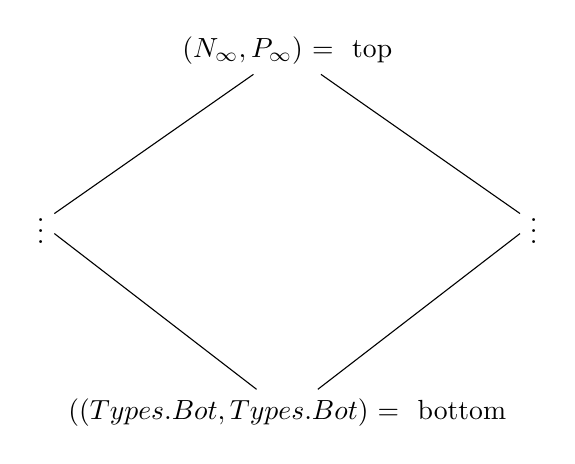
\begin{tikzpicture}[>=latex]

\node (top) {$\left(N_{\infty},P_{\infty}\right)$ = \text{ top}};

\node (left)  [below left=1.5cm and 1.5cm of top] {$\vdots$};
\node (right) [below right=1.5cm and 1.5cm of top] {$\vdots$};

\node (bottom) [below=4cm of top] { ($\left(Types.Bot,Types.Bot\right)$  = \text{ bottom}};
\draw (top) -- (left);
\draw (top) -- (right);
\draw (left) -- (bottom);
\draw (right) -- (bottom);

\end{tikzpicture}
\]

%% \tikzset{%
%%   draw seam allowance/.style 2 args={
%%     preaction={line width=1mm,line join=round,double distance=#1*2,draw=#2},
%%   },
%%   seam allowances/.style={%
%%     preaction={clip},
%%     preaction={draw seam allowance/.list={#1}},
%%     draw,%fill=white,
%%   },
%%   seam allowances/.default={{{2cm}{blue}}},
%%   invclip/.style={
%%     clip,
%%     insert path={
%%       {[reset cm] (-16000pt,-16000pt)  -| (16000pt,16000pt) -| cycle}
%%     },
%%   },
%% }
%% \begin{tikzpicture}
%%   \pgfmathsetseed{12}
%%   \foreach \X in {0,20,...,340}
%%   {\ifnum\X=0
%%   \xdef\mypath{(\X:2+rnd*0.9)}
%%   \else
%%   \xdef\mypath{\mypath (\X:2+rnd*0.9)}
%%   \fi
%%   }
%%   \begin{scope}
%%     \begin{pgfinterruptboundingbox}
%%       \path [invclip] \mypath;
%%     \end{pgfinterruptboundingbox}
%%     \draw [seam allowances={{4cm}{black},{2cm}{black}},line width=2mm]
%%     plot[smooth cycle] coordinates {\mypath };
%%   \end{scope}
%%   \node[font=\Huge] (a) at (9,9) {$x$};
%%     \draw[->,-{Latex[length=3mm]}] (a) -- ++(-120:5cm);  % 2 cm at -45°
%%     \node[font=\Huge] at (9,0) {$\nabla \mathrm{f(x)}$};
%%     \node[font=\Huge] at (0,9) {$ \mathrm{f(x)}$};
%% \end{tikzpicture}
%%
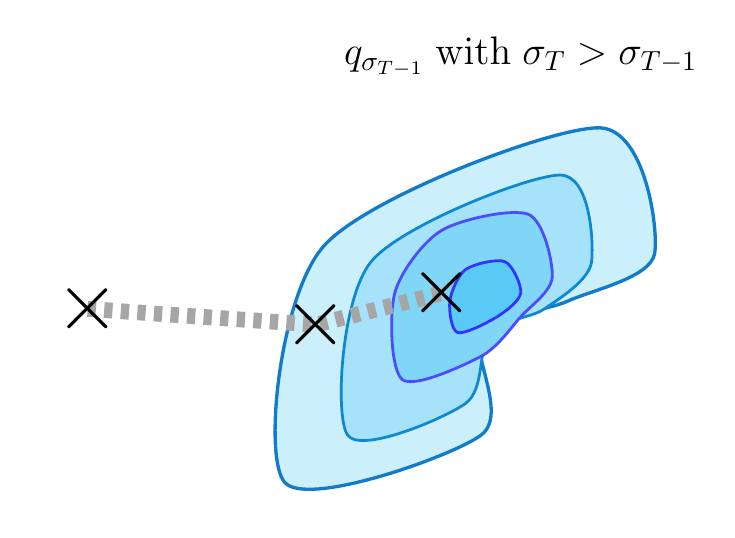
\begin{tikzpicture}[scale=1]

\filldraw[
fill=cyan!20,
draw=cyan!60!blue,
line width=1.2pt]
plot[smooth cycle]
coordinates{
(0.8,0.6)
(3.3,1.2)
(3.3,2.5)
(4.4,2.9)
(5.5,3.5)
(4.8,5.1)
(1.3,3.6)
};

\filldraw[
fill=cyan!35,
draw=cyan!70!blue,
line width=1pt]
plot[smooth cycle]
coordinates{
(1.6,1.2)
(3.1,1.6)
(3.4,2.5)
(4.1,2.8)
(4.7,3.4)
(4.3,4.5)
(1.9,3.4)
};

\filldraw[
fill=cyan!50,
draw=blue!70,
line width=1pt]
plot[smooth cycle]
coordinates{
(2.3,1.9)
(3.3,2.2)
(3.8,2.7)
(4.2,3.2)
(3.9,4.0)
(2.8,3.8)
(2.2,3.0)
};

\filldraw[
fill=cyan!65,
draw=blue!80,
line width=1pt]
plot[smooth cycle]
coordinates{
(3.0,2.5)
(3.5,2.7)
(3.8,3.0)
(3.6,3.4)
(3.1,3.3)
(2.9,2.9)
};

\draw[dashed,gray!70,line width=2mm]
(-1.7,2.8)--(1.2,2.6)--(2.8,3.0);

\node[scale=3] at (-1.7,2.8) {$\times$};
\node[scale=3] at (1.2,2.6) {$\times$};
\node[scale=3] at (2.8,3.0) {$\times$};

% Title
\node[font=\Large] at (3.8,6)
{$q_{\sigma_{T-1}}
\;\mathrm{with}\;
\sigma_T>\sigma_{T-1}$};

\end{tikzpicture}
\end{document}
